\subsubsection{Naming engine}

The naming engine turned out to be one of the most complex parts of the project. The naming engine is responsible for checking the names of various parts of the codebase, such as classes, methods, and variables and then converting them to match the user-defined configuration. The naming engine is split into multiple modules: the diagnostic module, code fix module; and the regex engine module. The diagnostic module is responsible for finding the issues in the codebase, the code fix module is responsible for fixing the issues, and the regex engine module is responsible for converting the names to match the user-defined configuration.

The diagnostic module uses the Roslyn API to parse the codebase and analyze objects, classes, methods, and variables. In order to reliably verify a name, the object name is check through the build-in C\# regex engine. If the name does not match the user-defined configuration, a diagnostic is created and added to the list of diagnostics that are returned to the user. The diagnostic is then displayed in the IDE, and the user can then choose to fix the issue.

The code-fix module acts as a wrapper for the regex engine, receiving the diagnostic from the diagnostic module and returning the corrected name.

As discussed in the prototype, a custom regex engine was necessary to allow for the conversion of the names to match the user-defined configuration. The regex engine is an instantiable object that when created is passed a regex pattern that will be used to match an input to.

The regex engine has three main functions: parse, convert, and match. The parse function is responsible for converting the regex pattern into a list of tokens, the convert function is responsible for converting the tokens into a tree structure, and the match function is responsible for matching the input to the tree structure.

\subsubsubsection{Pattern parsing}
During construction of the regex engine object, a regex pattern is to be provided which will be parsed into a token tree. The choice for representing the pattern data in a tree structure was made to allow for easy manipulation of the pattern. For example, if a quantifier token is found, it makes it significantly easier to determine what the quantifier token is linked to as we can either navigate up the tree or back one token to find the relevant token or set that needs to be quantified.
Due to current limitations with the regex parser, the regex pattern gets wrapped in a group construct, the reason for this is that the regex parser uses group constructs as the base token for the tree structure. All recognized token classes within this regex engine inherit from the base \texttt{AToken} abstract class which contains common properties and interfaces that all tokens must implement, this base class contains properties for the local pattern that the token represents, its parent, children, previous and next tokens in addition to the following abstract methods: \texttt{CanParse}; \texttt{Parse}; \texttt{Test}; and \texttt{Conform}. And the protected helper methods for recursively parsing children and reading individual tokens from a string.

\begin{wrapfigure}{r}{0.5\textwidth}
    \caption{Regex Token Recursive Parse}
    \label{fig:RegexTokenRecursiveParse}
    \centering
    \begin{subfigure}[b]{0.5\textwidth}
        \caption{Group Construct Recursive Parse}
        \label{fig:GroupConstructRecursiveParse}
        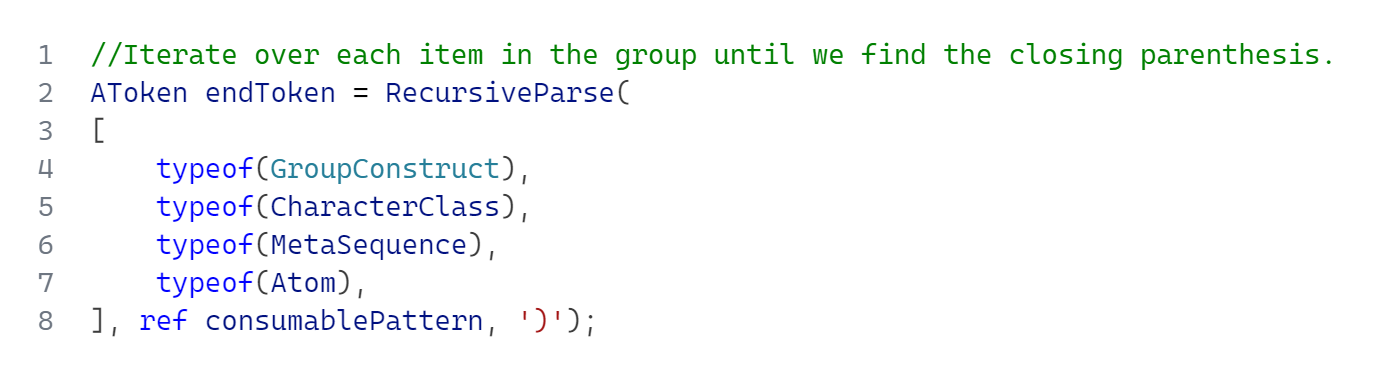
\includegraphics[width=\linewidth, height=0.3\textheight, keepaspectratio]{Figures/GroupConstructRecursiveParse.png}
    \end{subfigure}
    \begin{subfigure}[b]{0.5\textwidth}
        \caption{Recursive Token Parser}
        \label{fig:AToken_RecursiveParse}
        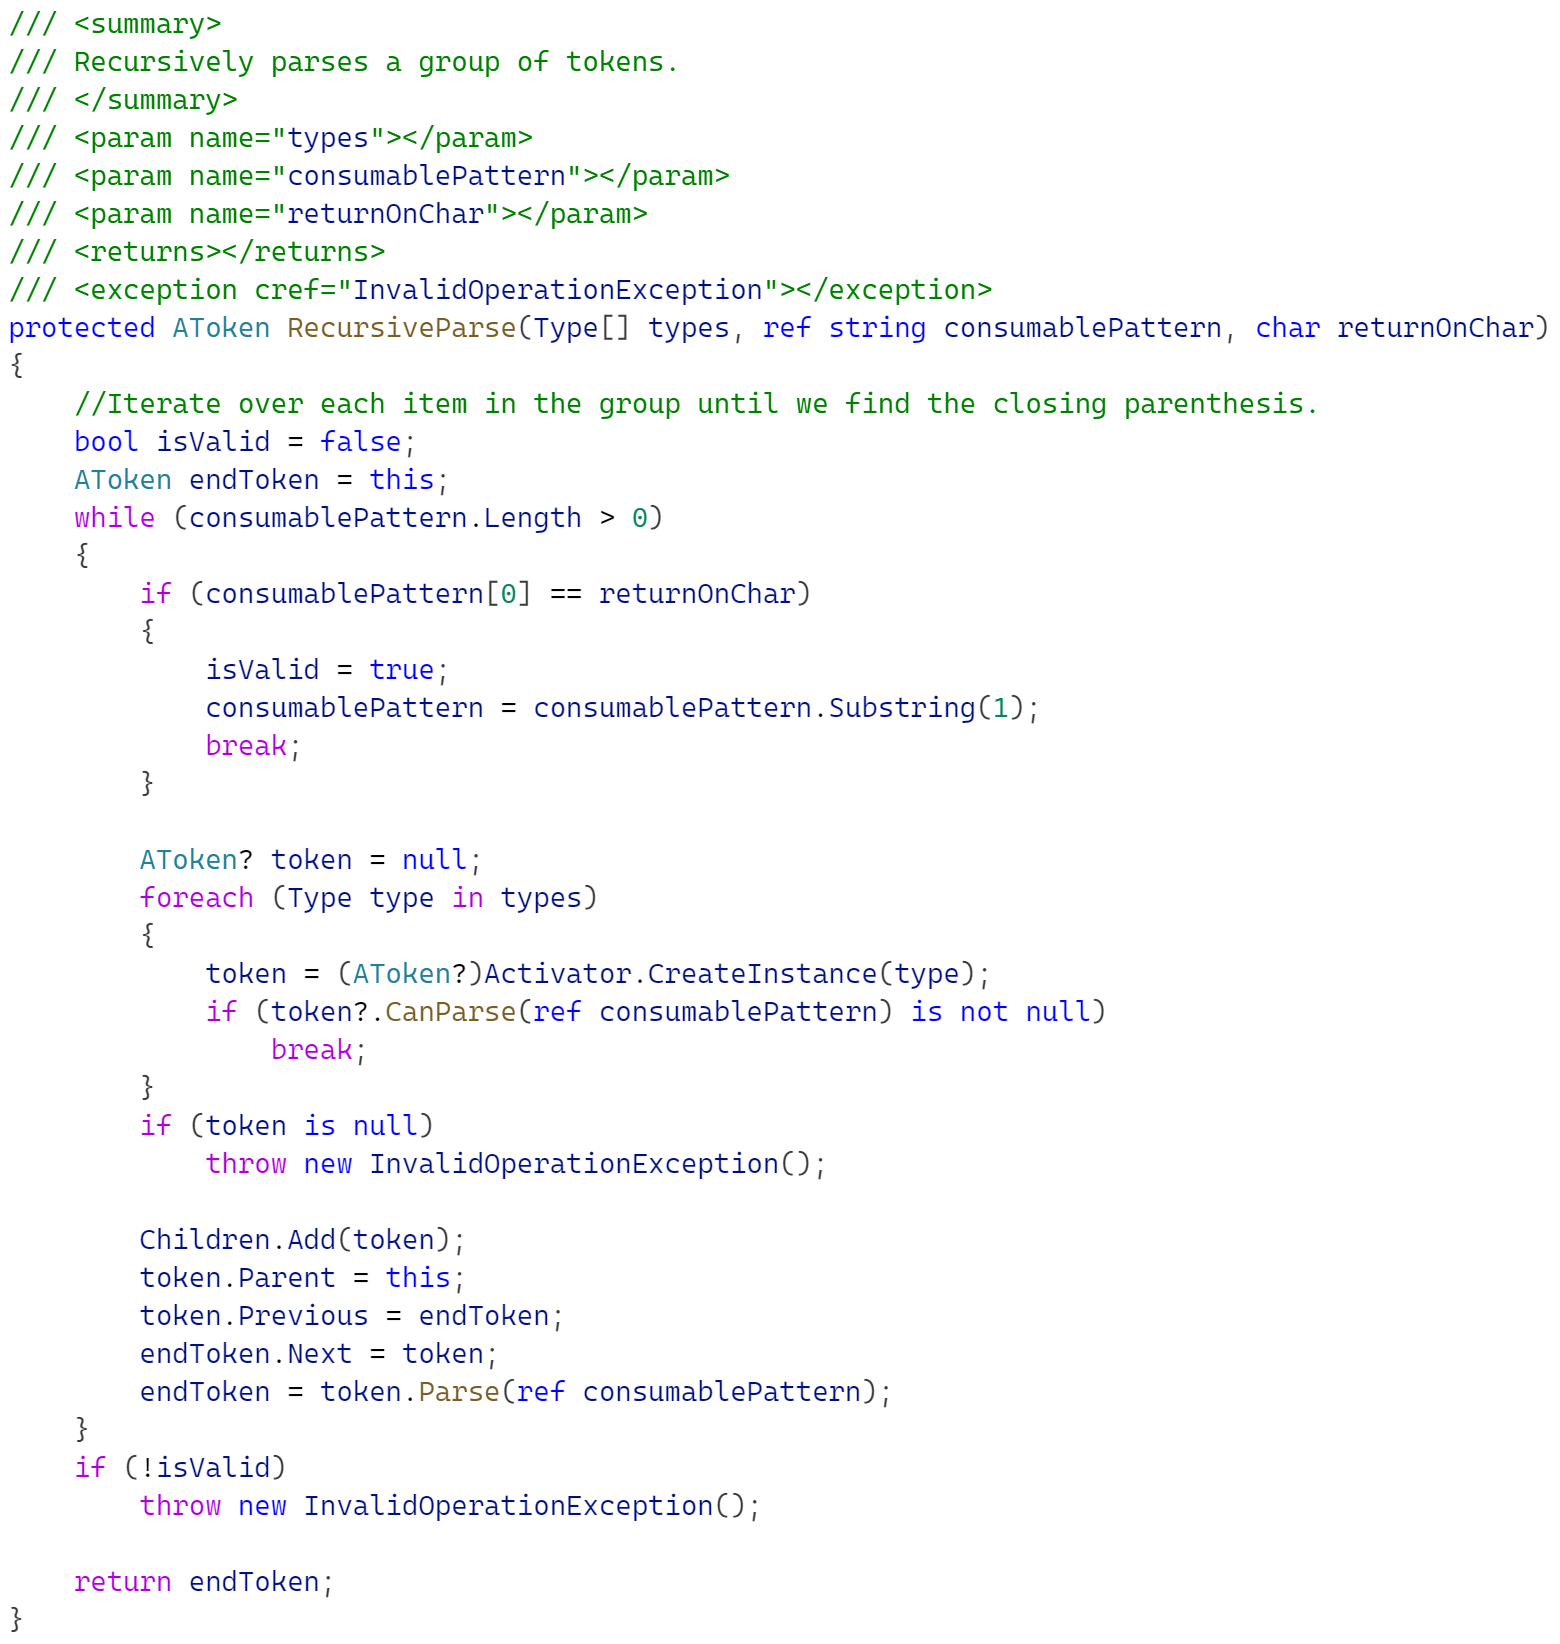
\includegraphics[width=\linewidth, height=\textheight, keepaspectratio]{Figures/AToken_RecursiveParse.png}
    \end{subfigure}
\end{wrapfigure}

The parse method is responsible for converting a pattern into a tree structure of tokens. Every token class has a different implementation of this method, for example, the group construct class will first check the construct type which could be for example a positive lookbehind. After this the helper, recursive parse method is called to parse the children within the group construct. This recursive parse method takes three parameters: a list of valid child tokens, a consumable pattern to parse, and a closing token to look for, the method will then proceed to consume the pattern and parse tokens (see figure \ref{fig:AToken_RecursiveParse}). For any valid tokens found a new instance of that token class is constructed and the parse method on that child will be called. After the child token has been parsed, the child tokens parent gets updated to the calling contexts token, the previous token of the child is set to the last token in the parent's children list, and the child token is added to the parent's children list. The method will then continue to consume the pattern until the closing token is found. If the closing token is not found, the method will throw an exception due to the pattern being invalid. If the closing token is found, the method will return the parsed tokens. The parse method is called recursively on the root token to parse the entire pattern into a tree structure of tokens.

\subsubsubsection{Input conversion}
The second part of the regex engine is the convert function. This function will attempt to convert an input string to conform to the pattern that the object was initialized with.
% TODO: Show the configuration options and what effect they have on the conversion.
Along with the input string, various options can be passed to the convert function to allow for fine-tuning of the conversion process. These options exist as there may be scenarios where certain parts of the pattern need to behave differently, for example, for literal tokens, the user may want to remove mismatched tokens or replace them with a valid token.
For the scenario of renaming code objects, we more often than not want to remove mismatched literals with a blank. To provide an example of this, if we want to conform the input \texttt{\_\_my\_variable} to the pattern \texttt{([A-Z][a-z]+)+}, it should produce a desired output of \texttt{MyVariable}. If mismatched tokens were not dropped the algorithm would fail to conform to the pattern as the pattern provides no way to match the literal characters \texttt{\_\_} to the pattern. By dropping these mismatched characters, the algorithm effectively ignores them from the output and matches where it can on valid tokens, producing an output of \texttt{MyVariable}.

The conversion process is a recursive process that starts at the root token of the tree structure. Each implementation of the abstract conform method takes a single parameter of the \texttt{ConformParameters} object, this object contains information about the current state of the conversion process, the input string, the current index in the input string, the current state of the newly generated output string and other options specific to other tokens.

The most complex operation in this process will be shown using the code from the \texttt{Quantifier} class. The quantifier parse method starts out by getting any quantifier options for the current index in the parsing process, this method will search up the tree for a quantifier token and return the options for that quantifier, the reason for this will become apparent later on. Following this the method will determine if the quantifier is greedy or not, within the conform parameters a value can be set to configure a greedy quantifier to break under certain conditions. The method will then attempt to run the conform method on its children, if the conform method fails the quantifier will break and return the current index in the input string if the quantifier was configured in the zero-or-more mode. After successfully parsing the children at least once, checks are then run to see if the quantifier should break, if it is greedy the quantifier will run until it can no longer match the pattern, if it is not greedy the quantifier will run either until the upper bound is reached or until the break condition is met. Currently this break condition allows for breaking on: character case changes; alphanumeric changes and delimiter changes. If the quantifier breaks the method will return the current index in the input string, if the quantifier does not break the method will return the index of the last successful match (see figure \ref{fig:QuantifierConformParameters}). The reason that the quantifier needed to initially search up the tree is because it needs to know its current context depth, if it is a nested quantifier then it should only conform to its local context and not a parent one, as the context is shared within the conform parameters object. When this method returns, the parent context will continue to parse the input string from the index that the quantifier has set within the conform parameters object.

\begin{figure}[H]
    \centering
    \caption{Quantifier Conform Parameters}
    \label{fig:QuantifierConformParameters}
    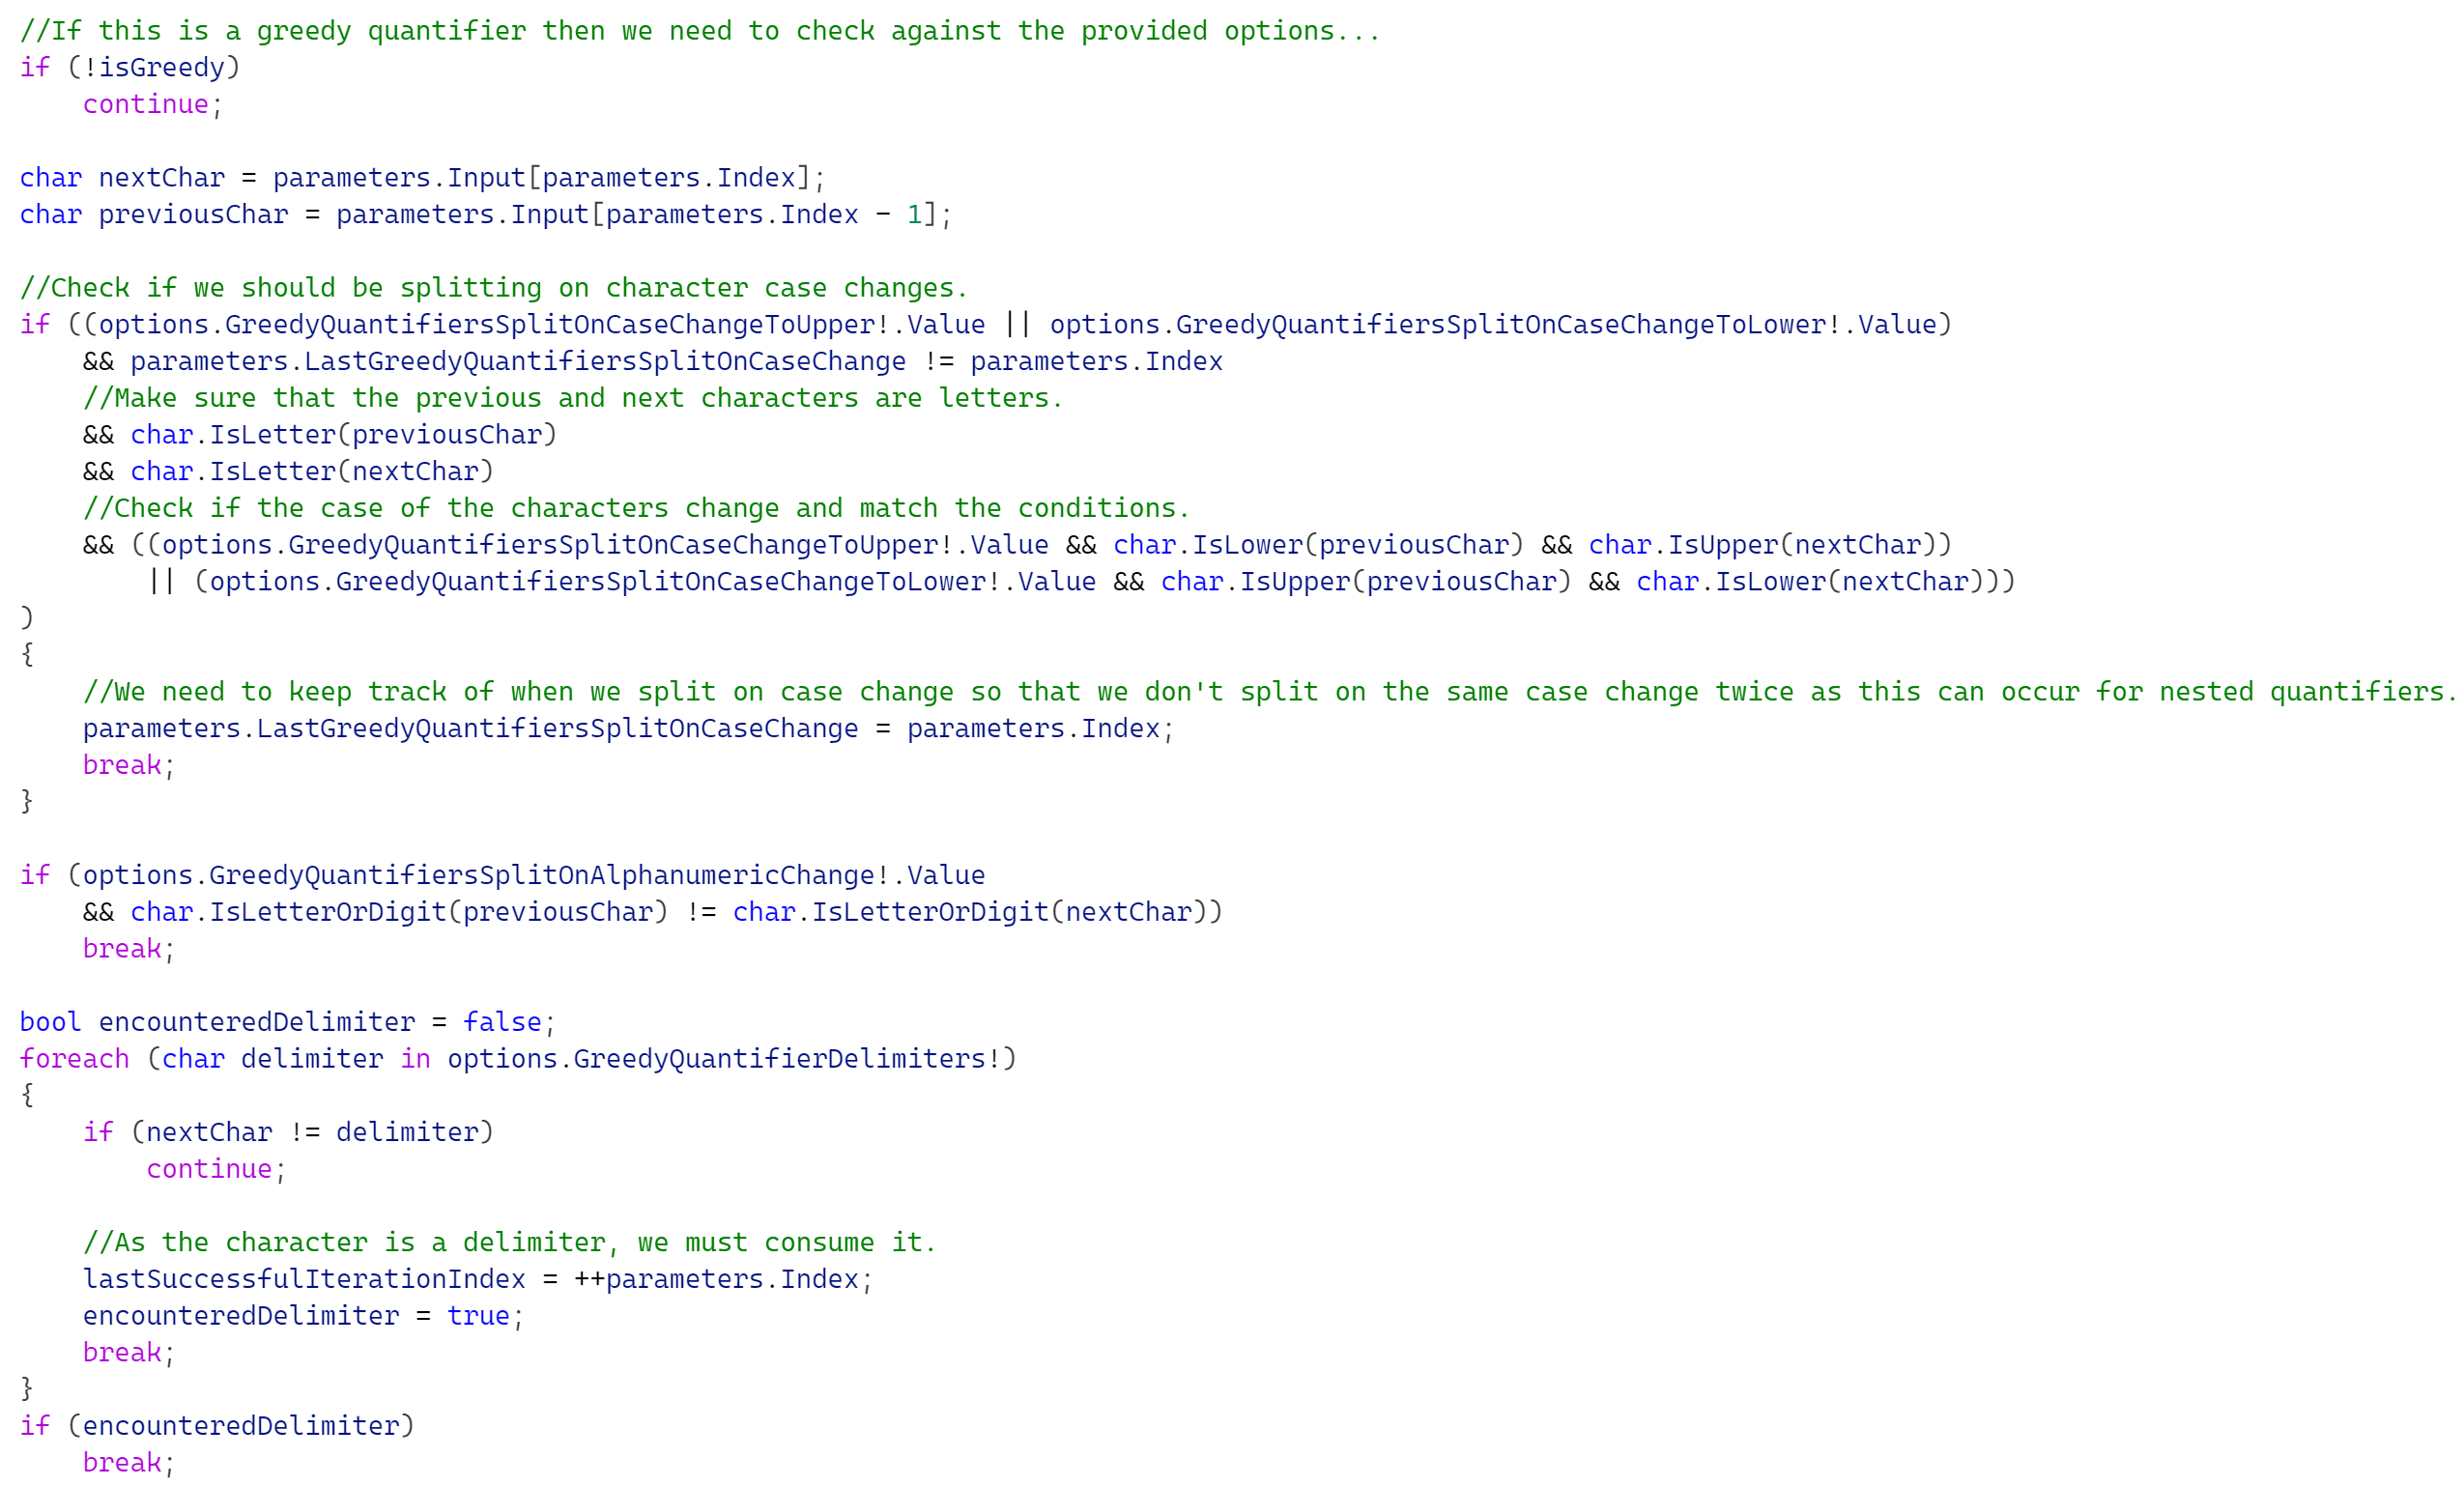
\includegraphics[width=1.0\textwidth]{Figures/QuantifierConformParameters.png}
\end{figure}

\begin{wrapfigure}{r}{0.5\textwidth}
    \centering
    \caption{Character Range Conform}
    \label{fig:CharacterRangeConform}
    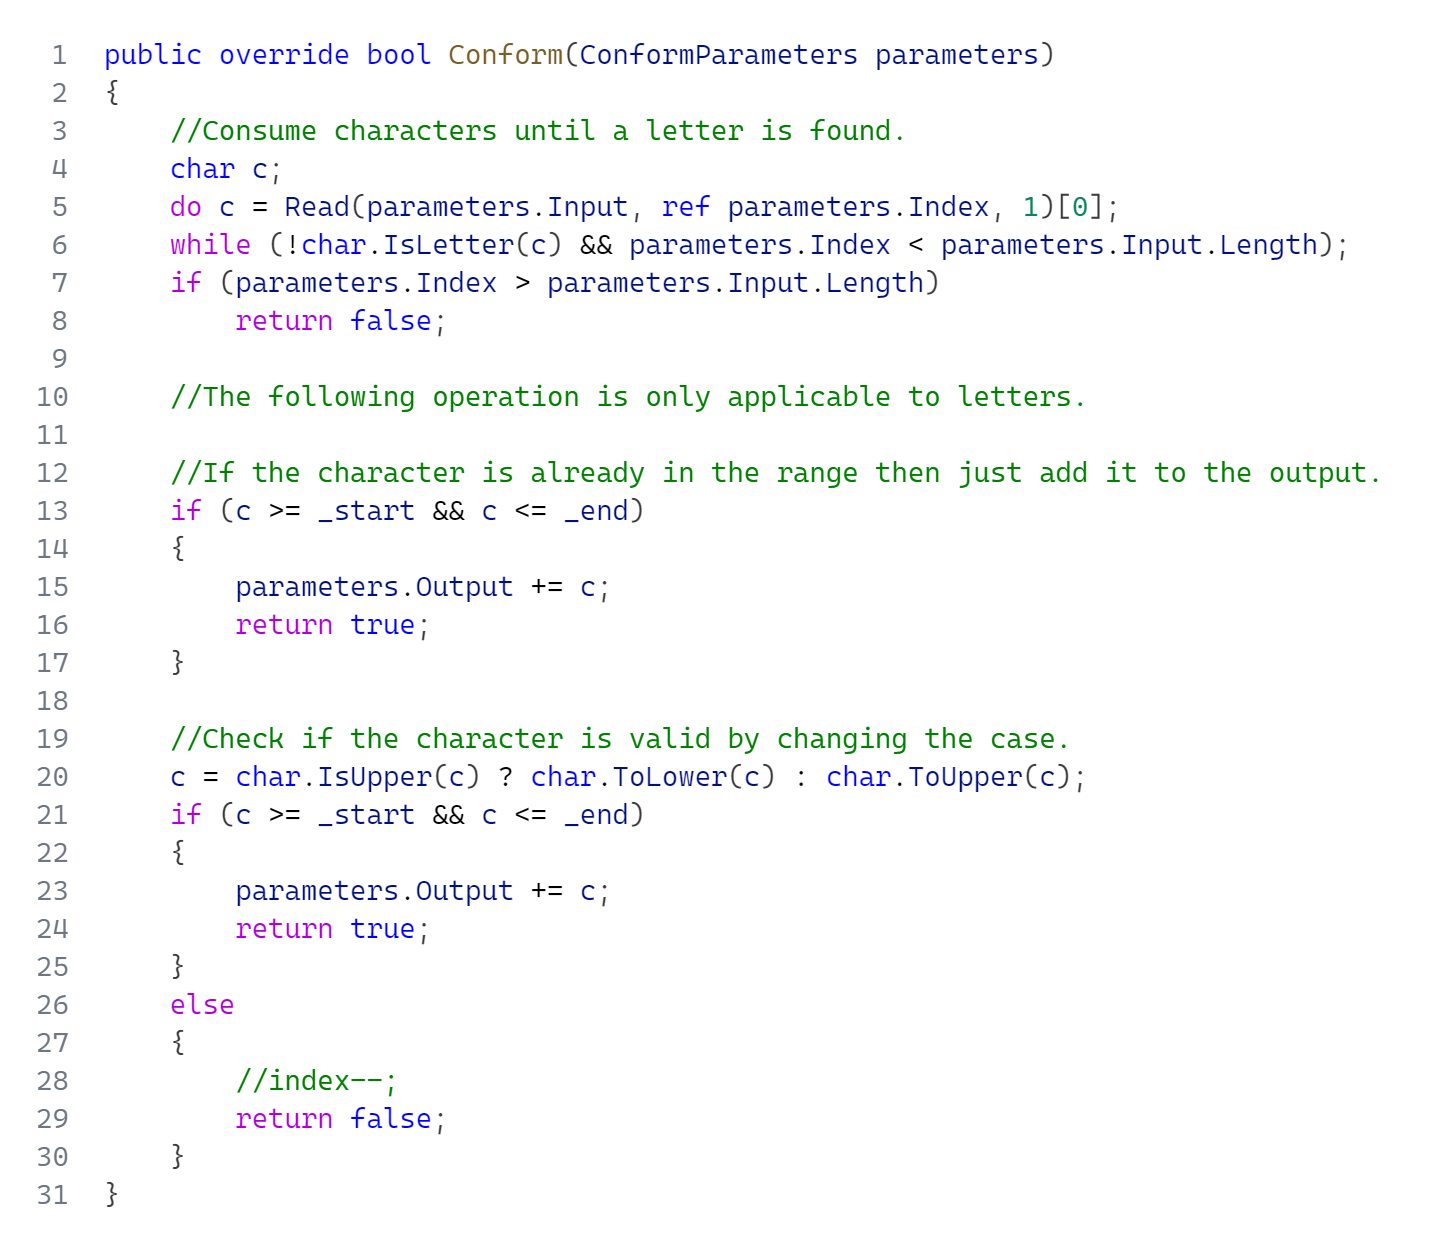
\includegraphics[width=0.5\textwidth]{Figures/CharacterRangeConform.png}
\end{wrapfigure}

To give an example of how an implementation of the conform method generates a corrected string, we can look at the \texttt{CharacterRange} class. The character range class in regex is used to match a single character to a range of valid characters. In the instance of this classes conform method. Firstly the character at the current index in the input string is checked to see if it is within the range of valid characters, this is achieved by comparing the characters unicode value to the unicode values of the start and end characters of the range. If the character is within the range, the character is added to the output string and the index is incremented. If the character is not within the range the method will attempt to see if the character can be converted to a valid character by changing the case of the character. For example if the valid range of characters was \texttt{[a-c]} and the input character was \texttt{A}, the method would convert the character to its lowercase variant and see if that character is within the range. If the character is within the range after the case change, the character is added to the output string and the index is incremented. If the character is still not within the range after the case change, the method will either drop the character if configured to do so, or return false indicating that it was unable to conform the input string to the pattern (see figure \ref{fig:CharacterRangeConform}).

\subsubsubsection{Output validation}
The final part of the regex engine is the match function. This function will validate wether the result from the conform function matches the pattern that the object was initialized with. Usually this function does not need to be called as the conform method will either succeed of fail. The method exists as a validation step to ensure that the output is correct for the provided pattern using the custom regex engine algorithm as it may possibly differ from the standard C\# regex engine.
% TODO: Show edge cases where this may be used.
